

\tikzset{every picture/.style={line width=0.75pt}} %set default line width to 0.75pt        

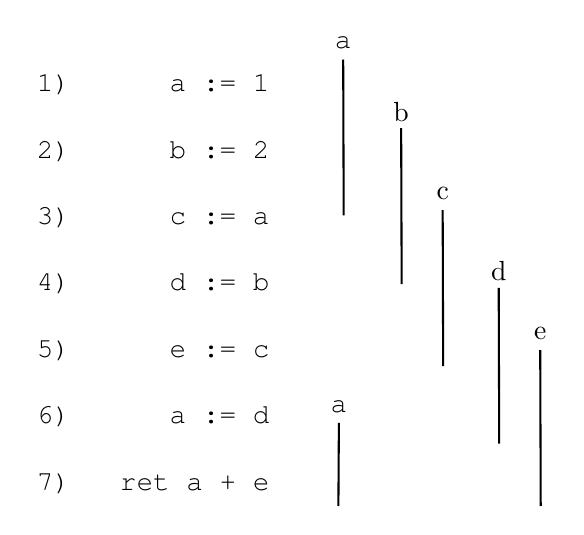
\begin{tikzpicture}[x=0.75pt,y=0.75pt,yscale=-1,xscale=1]
%uncomment if require: 
%\path (0,300); %set diagram left start at 0, and has height of 300

%Shape: Boxed Line [id:dp6151775546096955] 
\draw    (168.57,24.88) -- (168.81,100.02) ;


%Shape: Boxed Line [id:dp7225283089725557] 
\draw    (196.5,58) -- (196.74,133.14) ;


%Shape: Boxed Line [id:dp7093815356916122] 
\draw    (166.5,200) -- (166.26,240) ;


%Shape: Boxed Line [id:dp9729533201831728] 
\draw    (216.5,97.5) -- (216.74,172.64) ;


%Shape: Boxed Line [id:dp9278552127986968] 
\draw    (243.5,134.86) -- (243.74,210) ;


%Shape: Boxed Line [id:dp5443689225694379] 
\draw    (263.5,164.86) -- (263.74,240) ;



% Text Node
\draw (77,133) node  [align=left] {{\fontfamily{pcr}\selectfont 1) \ \ \ \ \ a := 1}\\\\{\fontfamily{pcr}\selectfont 2) \ \ \ \ \ b := 2}\\\\{\fontfamily{pcr}\selectfont 3) \ \ \ \ \ c := a}\\\\{\fontfamily{pcr}\selectfont 4) \ \ \ \ \ d := b}\\\\{\fontfamily{pcr}\selectfont 5) \ \ \ \ \ e := c}\\\\{\fontfamily{pcr}\selectfont 6) \ \ \ \ \ a := d}\\\\{\fontfamily{pcr}\selectfont 7) \ \ ret a + e}};
% Text Node
\draw (168.57,24.88) node  [align=left] {{\fontfamily{pcr}\selectfont a}\\};
% Text Node
\draw (196.5,58) node  [align=left] {b\\};
% Text Node
\draw (166.5,200) node  [align=left] {{\fontfamily{pcr}\selectfont a}\\};
% Text Node
\draw (216.5,97.5) node  [align=left] {c\\};
% Text Node
\draw (243.5,134.86) node  [align=left] {d\\};
% Text Node
\draw (263.5,164.86) node  [align=left] {e\\};


\end{tikzpicture}
